\documentclass[a4paper,12pt,oneside,onecolumn]{uerj}

\usepackage[brazil]{babel}  % adequacao para o portugues Brasil
\usepackage{cmap}           % Mapear caracteres especiais no PDF
\usepackage[utf8]{inputenc} % Determina a codificacao utiizada
                            % (conversão automática dos acentos)
\usepackage{makeidx}        % Cria o indice
\usepackage{hyperref}       % Controla a formacao do indice
\usepackage{lastpage}       % Usado pela Ficha catalografica
\usepackage{indentfirst}    % Indenta o primeiro paragrafo de cada secao.
\usepackage{color}          % Controle das cores
\usepackage{graphicx}       % Inclusao de graficos
\usepackage{amsmath,amssymb}        % pacote matemático
\usepackage{pdfpages}
\usepackage[top=3cm, bottom=2cm, left=3cm, right=2cm]{geometry}

\usepackage[frame=no,gride=no,algline=yes,font=default]{uerjformat}
\usepackage[alf]{abntcite}
\newcommand{\formato}[1]{\begin{flushleft}{#1}\end{flushleft}}
\newcommand{\BibTeX}{{{Bib}}\TeX}

\logo{uerj/logo_uerj_cinza.png}
\marcadagua{uerj/marcadagua_uerj_cinza.png}{1}{160}{255}


\instituicao{Universidade do Estado do Rio de Janeiro}
            {Centro de Tecnologia e Ciências}
            {Instituto de Matemática e Estatística}
            {Departamento de Informática e Ciência da Computação}

\autor{Juan}{Lopes}
\titulo{Expressões Regulares em Tempo Polinomial}

\orientador{titulação} % rotulo
           {[nome de]}{[sobrenome]} % {nome}{sobrenome}
           {[afiliação]} % afiliacao

\coorientador{titulação} % rotulo
           {[nome de]}{[sobrenome]} % {nome}{sobrenome}
           {[afiliação]} % afiliacao


\grau{Bacharel}
\curso{Informática e Tecnologia da Informação}

\local{Rio de Janeiro}   % cidade
\data{17}{Maio}{2013} % {dia}{mes}{ano}

% *****************************************************************************
% *****************************************************************************
% Configurações de aparência do PDF final
% *****************************************************************************
% *****************************************************************************

% alterando o aspecto da cor azul
%\definecolor{blue}{RGB}{41,5,195}

% informações do PDF
\hypersetup{
  %backref=true,
  %pagebackref=true,
  %bookmarks=true,                  % show bookmarks bar?
  pdftitle={\UERJtitulo},
  pdfauthor={\UERJautor},
  pdfsubject={\UERJpreambulo},
  pdfkeywords={Expressões Regulares}{Regex}{Autômatos Finitos},
  pdfproducer={LaTeX with class repUERJ}, % producer of the document
  pdfcreator={\UERJautor},
  colorlinks=true,                  % false: boxed links; true: colored links
  linkcolor=blue,                   % color of internal links blue
  citecolor=blue,                    % color of links to bibliography blue
  filecolor=blue,                % color of file links magenta
  urlcolor=blue,
  bookmarksdepth=4
}

\makeindex

\begin{document}

\frontmatter
\capa
\folhaderosto

%\includepdf{ficha_catalografica.pdf}

\begin{folhadeaprovacao}
  \assinatura{titulação membro1\\ afiliação1}
\end{folhadeaprovacao}

\pretextualchapter{Dedicatória}

  \vfill\vfill
    \hfill À minha esposa, Jacqueline.
  \vfill

% ----------------------------------------------------------
% Agradecimentos
% ----------------------------------------------------------

\pretextualchapter{Agradecimentos}

Texto de agradecimento.

% ----------------------------------------------------------
% Epigrafe
% ----------------------------------------------------------

\pretextualchapter{}

  \vfill\vfill\vfill\vfill
  \begin{flushright}
    Simplicity is a great virtue but it requires hard work to achieve it and education to appreciate it. And to make matters worse: complexity sells better.\\
    \textsl{Edsger W. Dijkstra}
  \end{flushright}
  \vfill

% ----------------------------------------------------------
% RESUMO
% ----------------------------------------------------------

\pretextualchapter{Resumo}

\refbibliografica

Este é o resumo em português.

\noindent {Palavras-chave}: Expressões regulares. Regex. Autômatos Finitos.

% ----------------------------------------------------------
% Abstract
% ----------------------------------------------------------

\pretextualchapter{Abstract}

This is the english abstract.

\noindent {Keywords}: Regular expressions. Regex. Finite automata.

\listadefiguras
\listadetabelas

\sumario

\mainmatter

%======================================================================================
\chapter{Introdução}
%======================================================================================

Neste capítulo serão apresentados a motivação, objetivos, e a estrutura do projeto.

%~~~~~~~~~~~~~~~~~~~~~~~~~~~~~~~~~~~~~~~~~~~~~~~~~~~~~~~~~~~~~~~~~~~~~~~
\section{Motivação}
%~~~~~~~~~~~~~~~~~~~~~~~~~~~~~~~~~~~~~~~~~~~~~~~~~~~~~~~~~~~~~~~~~~~~~~~

Expressões regulares fazem parte do ferramental da maioria das linguagens e plataformas de desenvolvimento modernas. Seu uso é bastante difundido na indústria para os mais variados fins, desde o reconhecimento de padrões, passando pela extração de símbolos para análise sintática de linguagens formais, até a sanitização de entradas do usuário para fins de segurança.

Seu extensivo uso vem precedido por uma forte base teórica na área de autômatos finitos, introduzida nos anos 40 por McCulloch e Pitts \cite{bib:McCulloch43}, formalizada na década seguinte por Kleene \cite{bib:Kleene56} e implementada por Ken Thompson no final dos anos 60 \cite{bib:Thompson68}, enquanto desenvolvia o editor de texto \emph{QED}, posteriormente portada para os mais conhecidos \emph{ed} e \emph{grep}, integrantes do sistema operacional Unix.



\begin{figure}[ht]
  \centering
  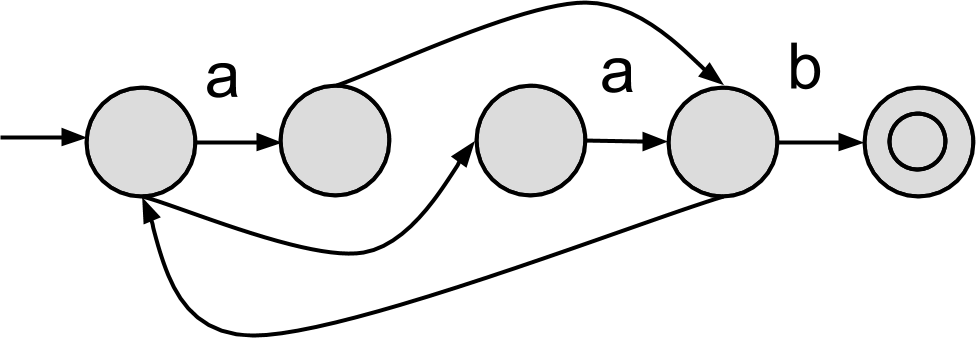
\includegraphics[scale=0.25]{figures/exemplo_automato.png}
  \caption{Exemplo de autômato para expressão regular (a\textbar b)+c}
\end{figure}


Desde então, conforme as implementações foram evoluindo, muitas funcionalidades foram adicionadas à linguagem de descrição de expressões regulares que as afastaram da teoria original. Enquanto originalmente descreviam linguagens estritamente regulares, a implementação mais difundida atualmente (\emph{PCRE}) é capaz não só de reconhecer qualquer linguagem livre de contexto, como também algumas sensíveis a contexto. \cite{bib:Nikita12}

Uma das consequências mais notáveis desta evolução não planejada é que o reconhecimento de strings da linguagem, um problema com solução linear originalmente, ganhou soluções exponenciais em um grande número de implementações modernas, que inclui muitas das mais usadas. Talvez a funcionalidade mais perigosa neste sentido sejam as backreferences, que não só impedem soluções polinomiais como tornam o problema de reconhecimento NP-completo. Entretanto, mesmo nas expressões que poderiam ser reconhecidas estritamente com autômatos finitos, certas particularidades de implementação as tornam potencialmente exponenciais, no pior caso. \cite{bib:Cox07}

Essas implementações tornam o uso de expressões regulares potencialmente inseguro em situações ora triviais. Um usuário mal intencionado pode ser capaz de forçar a execução de uma expressão com caráter exponencial para efetuar um ataque de negação de serviço em um servidor web, por exemplo. Muitas vezes a prevenção para esse tipo de ataque pode não ser trivial, e.g. em Java, onde métodos comumente usados contra a entrada do usuário, como \emph{replaceAll} e \emph{split}, da classe \emph{String} são implementados usado expressões regulares vulneráveis a esse tipo de ataque.

%~~~~~~~~~~~~~~~~~~~~~~~~~~~~~~~~~~~~~~~~~~~~~~~~~~~~~~~~~~~~~~~~~~~~~~~
\section{Objetivo}
%~~~~~~~~~~~~~~~~~~~~~~~~~~~~~~~~~~~~~~~~~~~~~~~~~~~~~~~~~~~~~~~~~~~~~~~

Este projeto tem dois objetivos principais. O primeiro é demonstrar através de testes pontuais e benchmarks os problemas fundamentais nas implementações de expressões regulares em diversas linguagens modernas, provando inclusive a NP-completude do problema de reconhecimento de strings nas linguagens que definem. O segundo objetivo é propor uma implementação didática e minimalista das expressões regulares propostas por Kleene, utilizando o método descrito por Thompson para construção e simulação do autômato. 

A implementação irá deixar de fora certas funcionalidades comuns nos \emph{sabores} mais modernos de expressão regular. Algumas destas funcionalidades podem ser implementadas sem sacrificar eficiência de execução. Outras, introduzem certa complexidade, porém mantendo a execução do algoritmo polinomial. O restante, entretanto, não é possível implementar sem tornar o algoritmo exponencial no pior caso. Todas as funcionalidades intencionalmente excluídas serão listadas e propostas de soluções serão apresentadas quando cabível.

Deseja-se mostrar com esse projeto que o problema de reconhecimento de expressões regulares pode ser resolvido de maneira eficiente, mesmo com as implementações mais simples, desde que seja observada a base teórica que as deu origem.

%~~~~~~~~~~~~~~~~~~~~~~~~~~~~~~~~~~~~~~~~~~~~~~~~~~~~~~~~~~~~~~~~~~~~~~~
\section{Estrutura}
%~~~~~~~~~~~~~~~~~~~~~~~~~~~~~~~~~~~~~~~~~~~~~~~~~~~~~~~~~~~~~~~~~~~~~~~

O projeto está divido em cinco capítulos. O capítulo 2 trata da base teórica por trás das expressões regulares, contando sua história, passando pelo método de construção do autômato de Thompson, e exibindo um algoritmo trivial (porém ineficiente) para sua solução.

O capítulo 3 descreve poder das implementações modernas de expressão regular, mostrando recursos avançados, como \emph{zero-width assertions} e \emph{backreferences}. Mostra também exemplos de expressões que reconhecem gramáticas não-regulares, exibindo o distanciamento entre estas e a teoria original. Por fim, é mostrado um benchmark comparando a performance entre as diversas implementações, que evidenciam uma diferença fundamental na forma como o problema é abordado em cada uma delas.

No capítulo 4 é proposta uma implementação de expressões regulares utilizando o método de Thompson. Os resultados teóricos e práticos desta implementação são discutidos e comparados com resultados anteriores.

O capítulo 5 expõe as conclusões e contribuições deste trabalho, bem como as dificuldades encontradas durante o projeto. Também serão listadas e descritas as funcionalidades não implementadas, possivelmente sugerindo formas eficientes de implementá-las, ou mesmo formas diferentes de simular o autômato que melhorem a eficiência geral da execução.

%======================================================================================
\chapter{Base Teórica}
%======================================================================================

AAA

\backmatter
%\citeoption{abnt-options4}
\bibliography{bibliografia}

\end{document}

